\documentclass{article}
\usepackage{cite}
\usepackage{graphicx} % Required for inserting images
\usepackage{float} % Make figures floatable
\usepackage{hyperref} % For referencing sections
% For making tables:
\usepackage{array}
\usepackage{booktabs}
\usepackage{longtable}

%% Adjusting Paper Document
\usepackage[a4paper, margin=1in]{geometry} % Adjust margins
\usepackage{setspace} % Adjust line spacing
\usepackage{titlesec} % Adjust spacing around sections
\usepackage{caption} % Adjust spacing around figures

\title{Deferral CSC8635 Machine Learning Project}
\author{Abdullah Turki H Alshadadi}
\date{}

% Set paragraph indentation to zero
\setlength{\parindent}{0pt}

% Reduce spacing between sections
\titlespacing\section{0pt}{10pt plus 2pt minus 2pt}{10pt plus 2pt minus 2pt}
\titlespacing\subsection{0pt}{8pt plus 2pt minus 2pt}{8pt plus 2pt minus 2pt}

% Reduce spacing around figures
% \setlength{\intextsep}{10pt plus 2pt minus 2pt}
% \setlength{\textfloatsep}{10pt plus 2pt minus 2pt}
% \setlength{\floatsep}{10pt plus 2pt minus 2pt}

% Adjust line spacing
\setstretch{1.1}

\begin{document}

\maketitle

\section{Introduction}

This report is about the image dataset task 2 in the CSC8635
Machine Learning Project. It will be structured in the typical
machine learning pipeline workflow, that is exploration, 
preprocessing, model training, model interpretation and 
evaluation.

\section{Exploration} \label{exploration}

The dataset being investigated is called CIFARTile, a 64x64
size images dataset which consist of 4 CIFAR-10 32x32 images as "tiles" in
the images. The labels corresponds to the number of unique CIFAR-10 
classification in an image minus 1, example images are in Figure \ref{fig:cifartile}.

\begin{figure}[H]
    \centering
    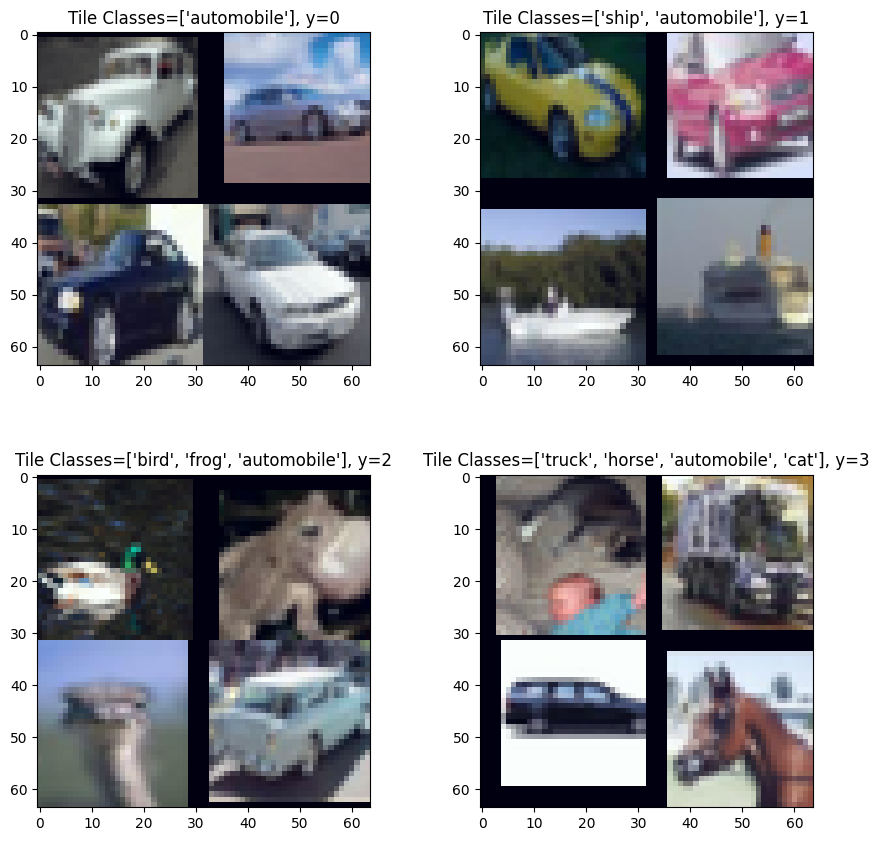
\includegraphics[width=0.7\linewidth]{images/cifartile.png}
    \caption{Examples of CIFARTile}
    \label{fig:cifartile}
\end{figure}

Investigating the distribution of labels across the dataset in 
Figure \ref{fig:dist_labels} shows that the data is well 
balanced which avoids instances of over-fitting or under-fitting.

\begin{figure}[H]
    \centering
    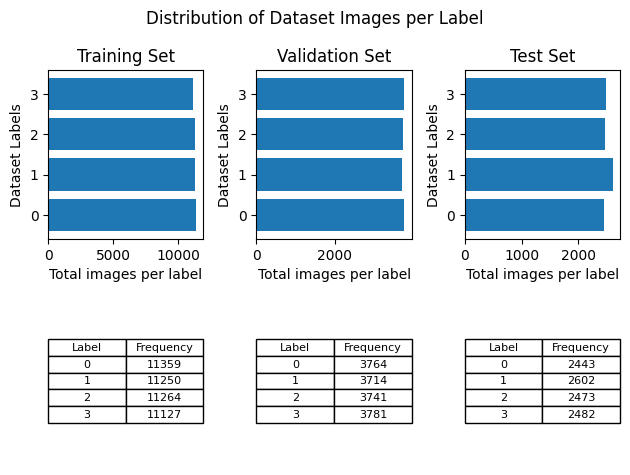
\includegraphics[width=0.7\linewidth]{images/dist_labels.png}
    \caption{The distribution of labels across the dataset}
    \label{fig:dist_labels}
\end{figure}

However, for the images in the dataset, the training and validation data
contain noise as in "empty black margins" between the CIFAR-10 images
in the CIFARTile (see Figure \ref{fig:org_img_train_valid}). On the
other hand the test data does not contain the same noise (see Figure
\ref{fig:test_img}). Furthermore, the images have non-standard colour
range scaling of -1.9892120361328125 to -1.9892120361328125.

\begin{figure}[H]
    \centering
    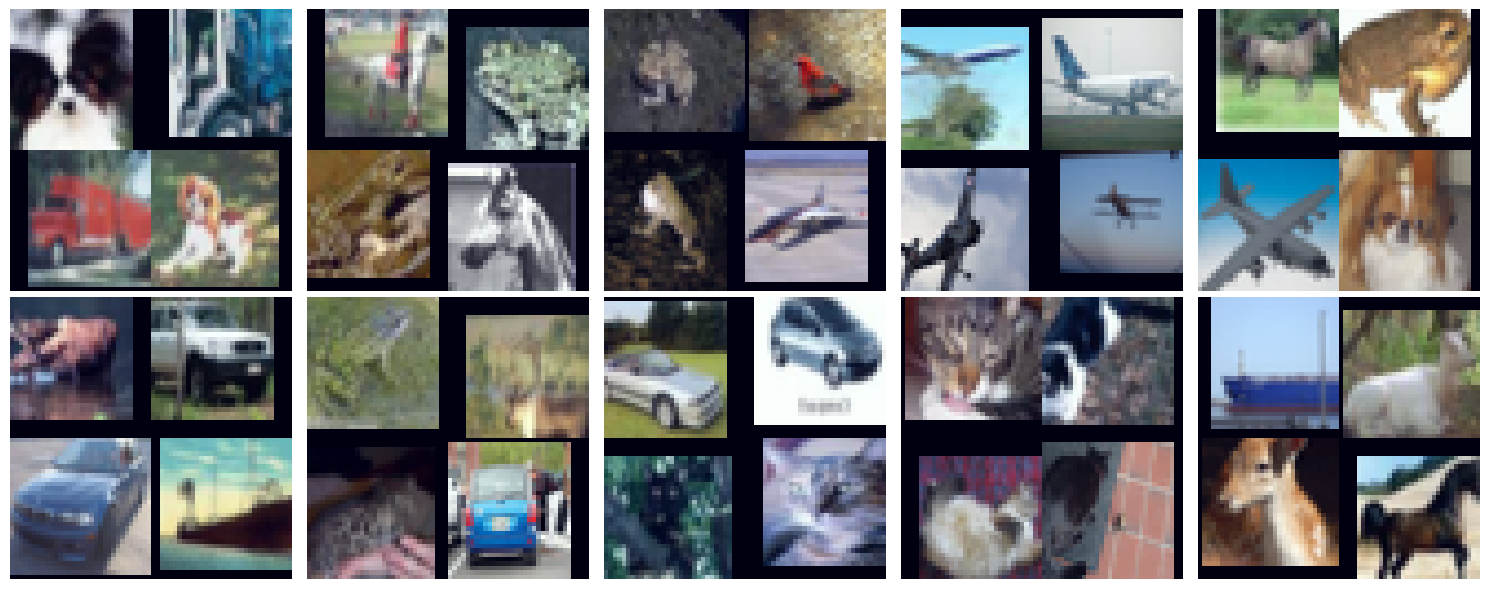
\includegraphics[width=0.7\linewidth]{images/org_img_train_valid.png}
    \caption{Example of the dataset images that contain "empty black margins"}
    \label{fig:org_img_train_valid}
\end{figure}

\begin{figure}[H]
    \centering
    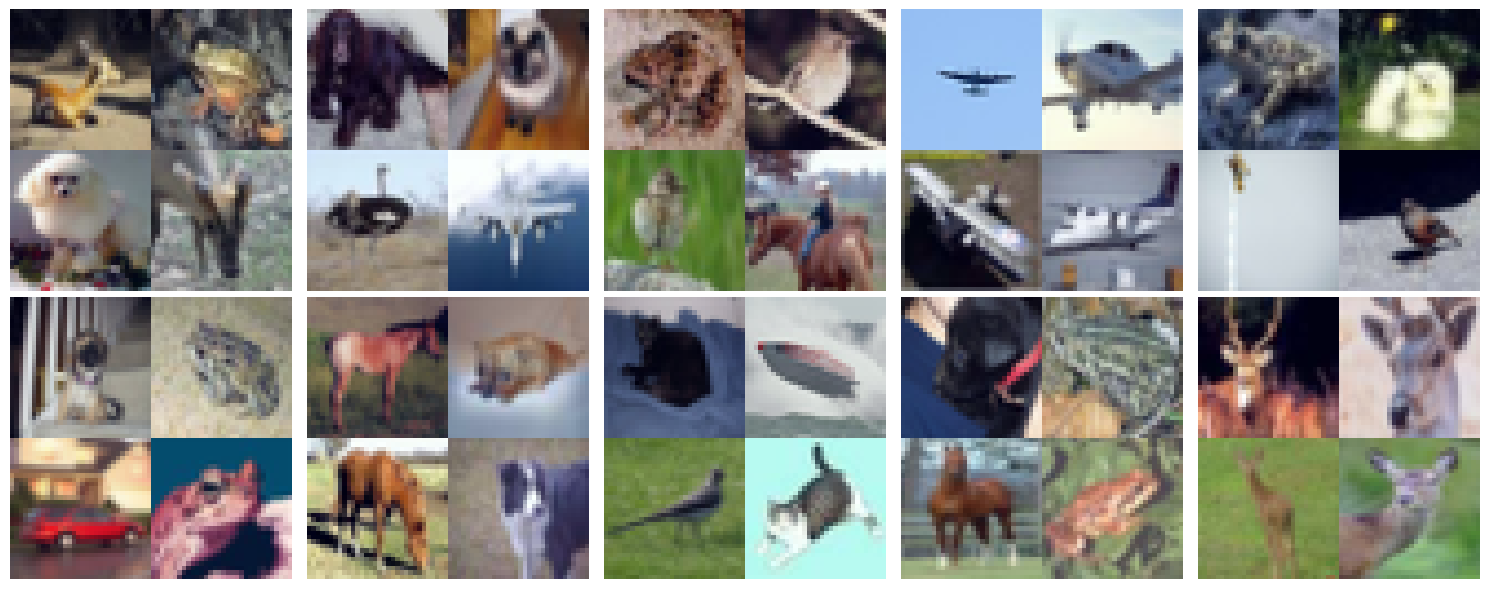
\includegraphics[width=0.7\linewidth]{images/test_img.png}
    \caption{Example of the test image which seems to not contain noise}
    \label{fig:test_img}
\end{figure}

\subsection{Finding the values of the noise}

In this subsection, the methodology took to identify the colour values of the
"empty black margins" noise.\\

First, use an image with the noise as the basis to finding the colour values. The
example used is the first image in the training data (see Figure 
\ref{fig:example_image_margins}). The image is then temporary 
converted to 8-bit 0 to 255 RGB colour values (see section 
\ref{preprocessing} Preprocessing for more details).

\begin{figure}[H]
    \centering
    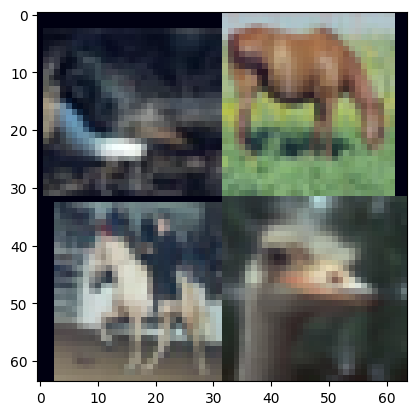
\includegraphics[width=0.7\linewidth]{images/example_image_margins.png}
    \caption{Base image used to identify the RGB 8-bit colour values of "empty black margins" noise}
    \label{fig:example_image_margins}
\end{figure}


Second, using the base image in Figure \ref{fig:example_image_margins}, the 
first row (top of the image), column (left vertical line) and last column (right vertical line) are retrieved then the mode is calculated to determine
the 3 channel colours which was determined to be \texttt{[0, 0, 17]}.\\

Last, to determine that the value is consistent with the other images in the dataset, 10 
images are randomly selected which then have every pixels set to white beside the pixels
containing the value \texttt{[0, 0, 17]}, see Figure \ref{fig:margin_detected} - you can see 
other pixels that are not noise have the same value as \texttt{[0, 0, 17]}, this is handled
in the section \ref{preprocessing} Preprocessing.

\begin{figure}[H]
    \centering
    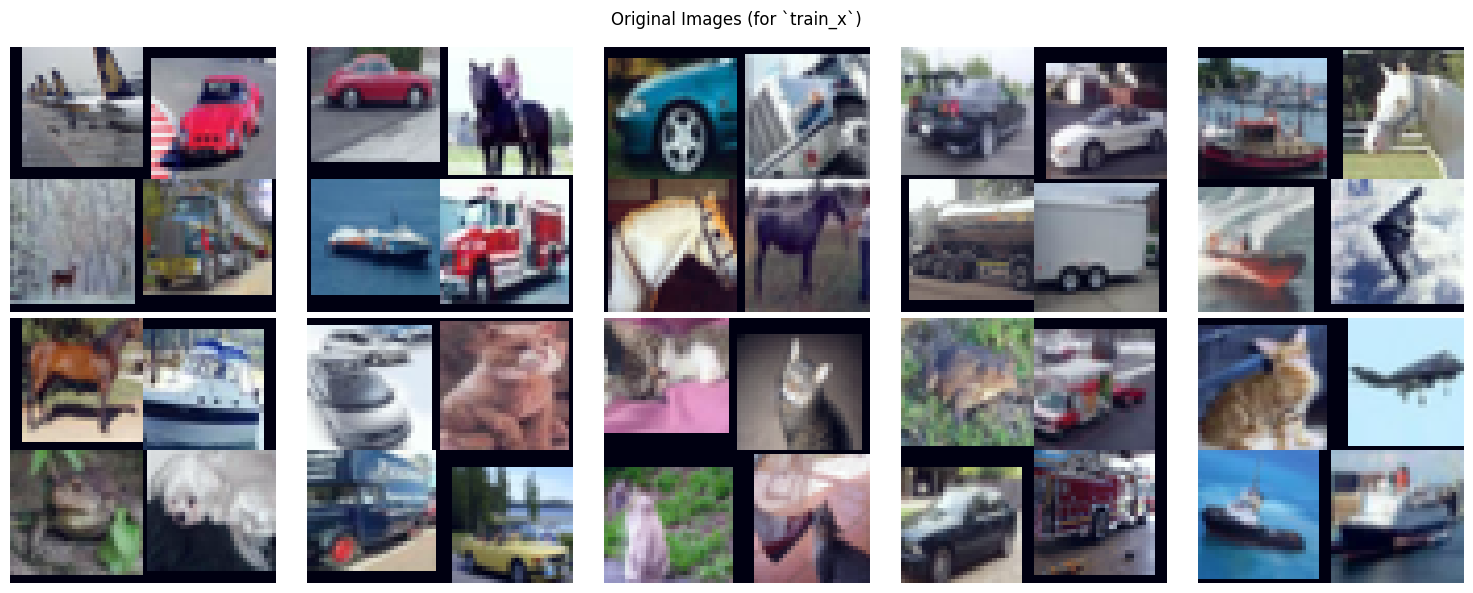
\includegraphics[width=0.7\linewidth]{images/org_img_before_detect_margin.png}
    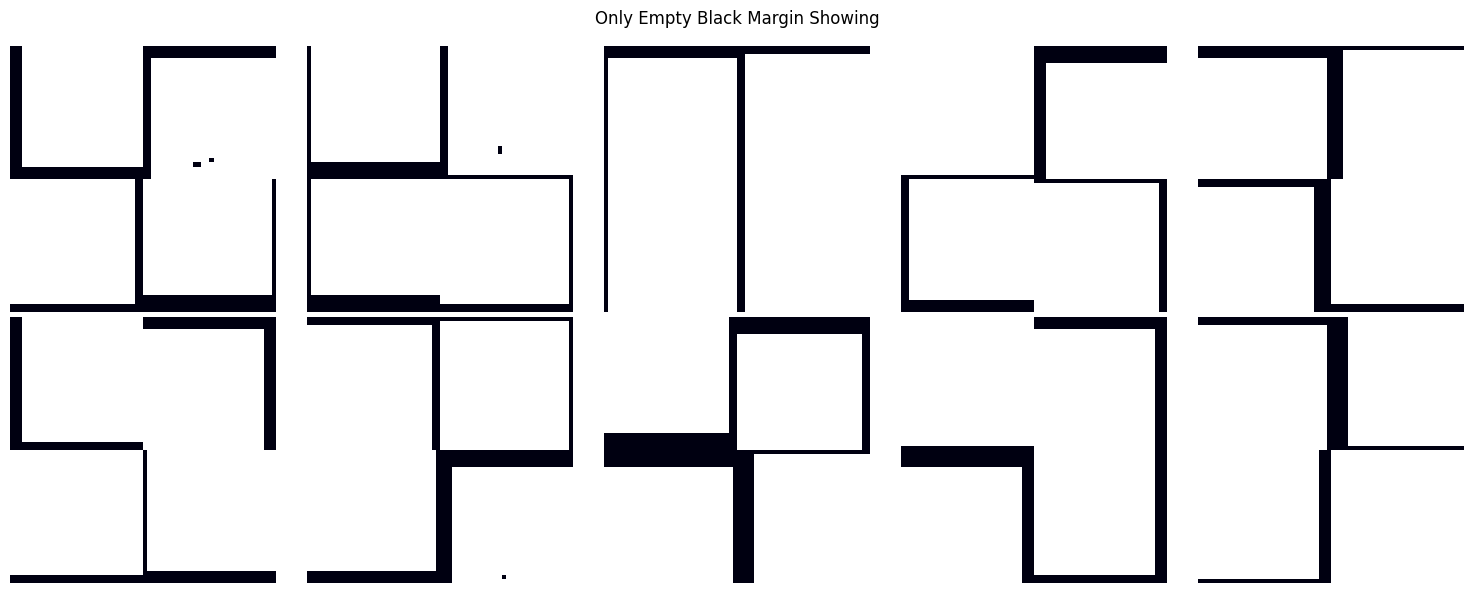
\includegraphics[width=0.7\linewidth]{images/margin_detected.png}
    \caption{10 random images that shows the original images compare to only keeping the values \texttt{[0, 0, 17]}}
    \label{fig:margin_detected}
\end{figure}

\section{Preprocessing} \label{preprocessing}

In this section, it will discuss how is the noise removed in the images
(subsection \ref{preprocess_noise}) and how are the labels handled 
(subsection \ref{handle_labels}).

\subsection{Removing noise in the images} \label{preprocess_noise}

First, the image is normalised from the colour range scaling of 
-1.9892120361328125 to -1.9892120361328125, to a 0 to 1 scaling. Then it will 
be further scaled to unsigned 8-bit integer scaling of 0 to 255 which 
done in the reason of simplify the preprocessing preprocess of removing 
the noise in images.\\

Second, a Python class called \texttt{EmptyMarginRemover} which contain
the functions \texttt{split\_tiles()},\\ \texttt{remove\_empty\_margins()},
\texttt{combine\_tiles()} and \texttt{preprocess()}.\\

The \texttt{preprocess()} is the main function that runs the 
\texttt{EmptyMarginRemover} class, which takes 64x64 unsigned 8-bit 
RGB channel CIFARTile images and it will be fed to other functions
of the class in this order:  \texttt{split\_tiles()}, \texttt{remove\_empty\_margins()},
\texttt{combine\_tiles()}.\\

As discussed in section \hyperref[exploration]{Exploration}, the CIFARTile
dataset consists of 4 CIFAR-10 images which is divided into 32x32 images in
the 64x64 image - this is further confirmed by looking at the test data, 
see Figure \ref{fig:test_img}. Thus, the CIFARTile images are split into
4 images by the \texttt{split\_tiles()} function to simplify the preprocessing
methodology.\\

The 4 images are then fed individually into the \texttt{remove\_empty\_margins()}
function. This function takes each row and column of the images and 
calculates the average of each colour values to determine if the row
or column pixels only contain the values of \texttt{[0, 0, 17]} which 
has the average of 6 when rounded as a whole number (see Figure
 \ref{fig:remove_margin_equation}).

\begin{figure}[H]
    \centering
    \captionsetup{justification=centering}
    \begin{equation}
        row\_or\_column\_of\_pixels\_in\_a\_tile = 32
    \end{equation}
    \begin{equation}
        colour\_channel\_of\_empty\_margin = (0 + 0 + 17)
    \end{equation}
    \begin{equation}
        rgb\_colour\_channel\_size = 3
    \end{equation}
    \begin{equation}
        total\_pixels\_with\_colour\_channels = row\_or\_column\_of\_pixels\_in\_a\_tile \times rgb\_colour\_channel\_size
    \end{equation}
    \begin{equation}
        \frac{row\_or\_column\_of\_pixels\_in\_a\_tile \times colour\_channel\_of\_empty\_margin}{total\_pixels\_with\_colour\_channels} = 5.6666666\ldots
    \end{equation}
    \begin{equation}
        \frac{32 \times (0 + 0 + 17)}{(32 \times 3)} = 5.6666666\ldots
    \end{equation}
    \caption{Equations related to tile processing}
    \label{fig:remove_margin_equation}
\end{figure}

Once each of the 4 images are preprocessed under 
\texttt{remove\_empty\_margins()} function, it will then be combined
back into 64x64 CIFARTile using \texttt{combine\_tiles()} and returned - 
see examples of before and after the preprocessing in Figure \ref{fig:before_and_after_preprocess}

\begin{figure}[H]
    \centering
    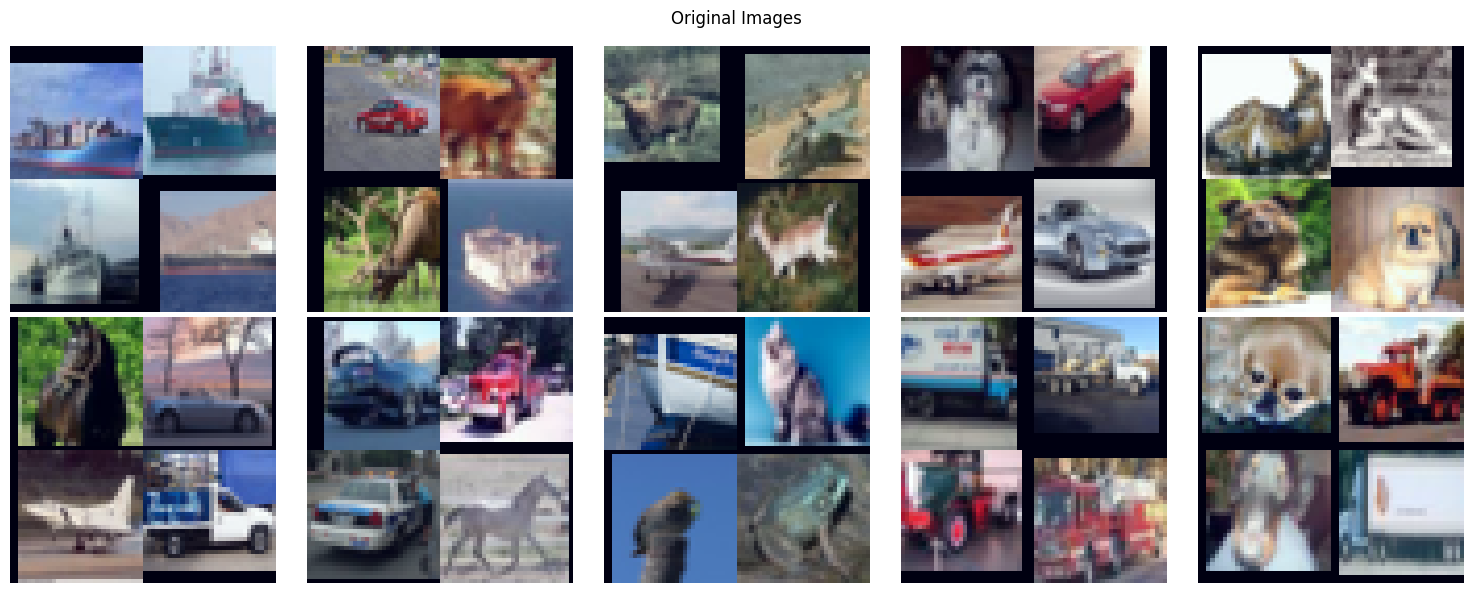
\includegraphics[width=0.7\linewidth]{images/before_preprocess.png}
    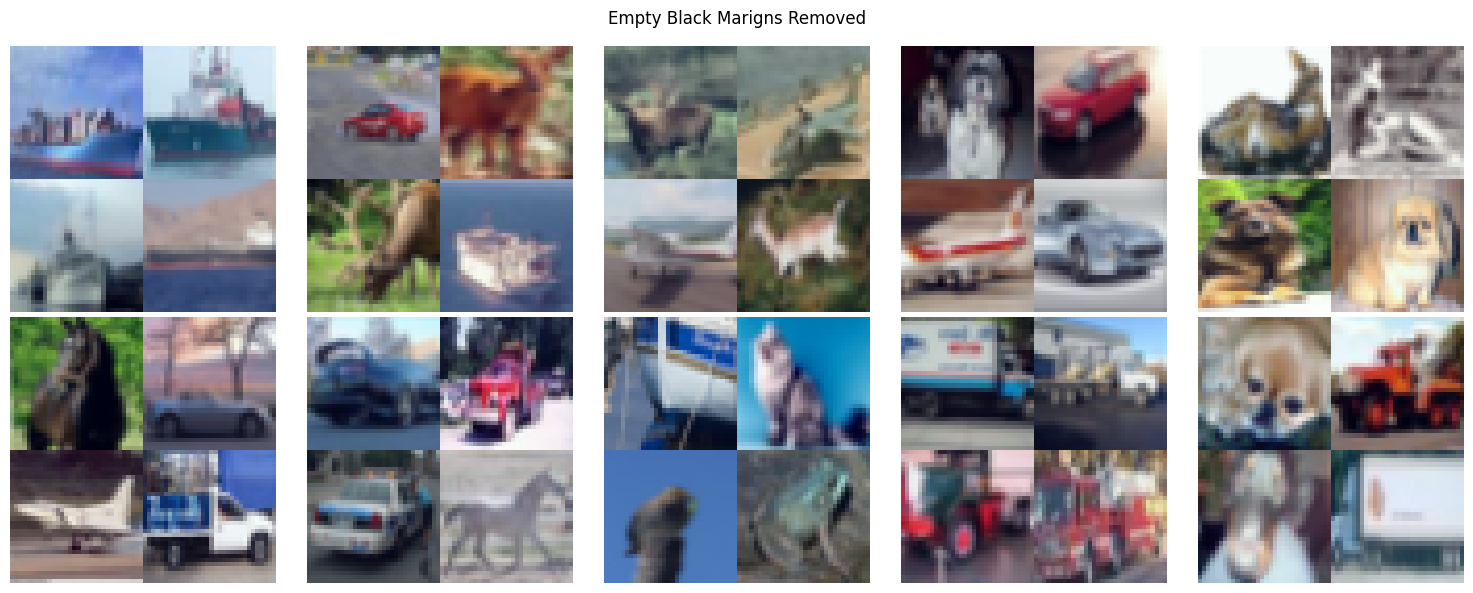
\includegraphics[width=0.7\linewidth]{images/after_preprocess.png}
    \caption{Example of image before and after the \texttt{EmptyMarginRemover} preprocess class}
    \label{fig:before_and_after_preprocess}
\end{figure}

\subsection{Handling labels} \label{handle_labels}

Due to this being a image classification problem, one-hot encoding is
performed on the labels to provide the model more information of the 
categorical variables.

\section{Model Training} \label{model training}

\subsection{Why ResNet50v2?}

ResNet50v2 is well-suited for the CIFARTile image classification problem 
due to its architectural strengths and proven performance in complex 
image tasks \cite{7780459, DBLP:journals/corr/HeZR016}.\\

Firstly, the depth of ResNet50v2, comprising 50 layers, enables it to 
learn and represent complex patterns effectively. This depth is crucial 
for the CIFARTile dataset, where each 64x64 image consists of four tiled 
CIFAR-10 images, creating a more complex classification challenge than 
standard single-image tasks.\\

A key feature of ResNet architectures, including ResNet50v2, is residual
connections. These connections help prevent the vanishing gradient problem,
facilitating efficient training even with many layers. This is particularly 
beneficial for CIFARTile images, where capturing intricate features across 
the tiled sub-images is essential.\\

ResNet50v2 is designed to capture hierarchical features, starting from
low-level features such as edges and textures to high-level features 
like shapes and objects. This ability to capture and integrate features 
at different scales is crucial for accurate classification of CIFARTile 
images, which contain multiple smaller images.\\

ResNet50v2 has a strong track record in image classification benchmarks,
demonstrating high accuracy and robustness across diverse datasets. 
Its proven performance on the CIFAR-10 dataset, which forms the basis 
of the CIFARTile dataset, underscores its reliability for extending 
to the more complex CIFARTile problem.\\

In summary, ResNet50v2’s depth, residual connections, hierarchical
feature learning, proven effectiveness, and adaptability make it
an excellent choice for the CIFARTile classification task.

\subsection{Hyperparameter tuning}

For the Hyperparameter tuning, a grid-search is used to iterate to all
possible hyperparameter combinations. The hyperparameters chosen are the following:

\begin{table}[h]
    \centering
    \begin{tabular}{@{} lll @{}}
        \toprule
        \textbf{Pooling} & \textbf{Optimizer} & \textbf{Learning Rate} \\
        \midrule
        avg             & adam               & 0.1            \\
        max             & rmsprop            & 0.01           \\
                        & sgd                & 0.001          \\
        \bottomrule
    \end{tabular}
    \caption{Configuration hyperparameters for the model}
    \label{tab:config_hyperparameter}
\end{table}

The choice of hyperparameters for ResNet50v2 aims to optimise its 
performance for the CIFARTile image classification task by exploring 
various configurations.\\

For pooling methods, average pooling (avg) smooths feature maps
by averaging values within a pooling window, reducing noise and 
retaining prominent features. This helps stabilise the learning 
process. On the other hand, max pooling (max) selects the maximum 
value in a pooling window, capturing dominant features and preserving 
important spatial hierarchies, which is useful for well-defined features.\\

Regarding optimisers, Adam combines the benefits of AdaGrad and RMSProp, 
adapting learning rates for each parameter, making it robust and efficient
for training deep networks. RMSprop adjusts learning rates based on an
exponentially decaying average of squared gradients, which stabilises
training and speeds up convergence. Stochastic Gradient Descent (SGD)
updates model parameters in the direction of the negative gradient and
is effective with momentum for large-scale problems, helping to escape
local minima and converge to the global minimum.\\

The learning rates chosen are 0.1, 0.01, and 0.001. 
A high learning rate of 0.1 allows for faster convergence 
but carries the risk of overshooting. A moderate rate of 0.01
balances speed and accuracy, providing stable updates. A low rate
of 0.001 ensures precise convergence, reducing the risk of overshooting,
making it ideal for fine-tuning.\\

This systematic exploration of pooling methods, optimisers, and 
learning rates helps identify the best hyperparameter combination, 
ensuring robust and accurate classification for the CIFARTile dataset.

\section{Model Interpretation and Evaluation} \label{evaluation}

\subsection{Interpreting the hyperparameter tuning}

\begin{longtable}{|l|l|l|l|l|l|}
    \hline
    \textbf{Trial} & \textbf{Pooling} & \textbf{Optimizer} & \textbf{Learning Rate} & \textbf{Validation Accuracy} \\ \hline
    \endfirsthead
    \hline
    \textbf{Trial} & \textbf{Pooling} & \textbf{Optimizer} & \textbf{Learning Rate} & \textbf{Validation Accuracy} \\ \hline
    \endhead
    0002 & avg & adam & 0.001 & 0.525 \\ \hline
    0005 & avg & rmsprop & 0.001 & 0.524 \\ \hline
    0003 & avg & rmsprop & 0.01 & 0.449 \\ \hline
    0000 & avg & adam & 0.01 & 0.435 \\ \hline
    0016 & max & sgd & 0.1 & 0.424 \\ \hline
    0007 & avg & sgd & 0.1 & 0.421 \\ \hline
    0011 & max & adam & 0.001 & 0.403 \\ \hline
    0015 & max & sgd & 0.01 & 0.386 \\ \hline
    0006 & avg & sgd & 0.01 & 0.386 \\ \hline
    0017 & max & sgd & 0.001 & 0.277 \\ \hline
    \caption{Summary of the 10 Best Trials}
    \label{tab:top_10_trials}
\end{longtable}

The results of the best 10 trials indicate that the optimal configuration
for the ResNet50v2 model on the CIFARTile dataset involves specific
combinations of hyperparameters.\\

The most successful trial (0002) used an Adam optimiser with a 
learning rate of 0.001 and average pooling, achieving the highest score 
of 0.525. This suggests that Adam with a low learning rate and average 
pooling is highly effective.\\

Trial 0005, with similar settings but using RMSprop 
instead of Adam, achieved a nearly equivalent score of 0.524,
indicating that RMSprop is also a strong choice when paired with
average pooling and a low learning rate.\\

Scores declined notably when the learning rate was increased to 0.01,
as seen in trials 0003 and 0000, regardless of whether Adam or RMSprop 
was used, showing the importance of a lower learning rate for optimal 
performance.\\

Trials with max pooling generally performed worse than those with
average pooling. For instance, trial 0011, which used max
pooling with Adam and a learning rate of 0.001, had a lower
score of 0.403.\\

SGD as an optimiser, regardless of the pooling method or learning rate,
consistently yielded lower scores compared to Adam and RMSprop.
The best SGD result (trial 0016) with max pooling and a learning rate
of 0.1 scored 0.424, further emphasising that SGD is less effective for
this task.\\

Overall, the results highlight that using the Adam optimiser
with a learning rate of 0.001 and average pooling provides the best
performance for the ResNet50v2 model on the CIFARTile dataset.

\subsection{Evaluating the best 2 models}

two best models from the trials, namely Trial 0002 and Trial 0005,
Both models exhibit similar performance, but there are slight 
differences in their metrics. Trial 0005 achieves a marginally
higher test accuracy (50.58\%) compared to Trial 0002 (50.37\%).
This indicates that Trial 0005 correctly classifies a slightly
higher percentage of test samples.\\

However, when considering precision, Trial 0002 (0.4995) outperforms
Trial 0005 (0.4896). Precision measures the accuracy of positive
predictions, suggesting that Trial 0002 is somewhat better at ensuring
that predicted positives are actual positives.\\

In terms of recall, which measures the ability to capture actual
positives, Trial 0005 (0.5058) is marginally better than Trial 0002
(0.5037). This means Trial 0005 is slightly more effective at identifying
true positive cases.\\

For confusion matrix, see Figure \ref{fig:confusion_matrix}, The confusion 
matrix indicatesstrong performance in label class \texttt{1} and \texttt{2}
for Trail 0002, however, it is worser classification for labels 
\texttt{0} and more worse \texttt{4} compare to Trail 0005.\\

The F1 Score, which balances precision and recall,
is slightly higher for Trial 0002 (0.4988) compared
to Trial 0005 (0.4878). This indicates that Trial 0002 has
a more balanced performance between precision and recall despite,
Trial 0002 having a weaker classification for class label 
\texttt{4} than Trial 0005.

\begin{figure}[H]
    \centering
    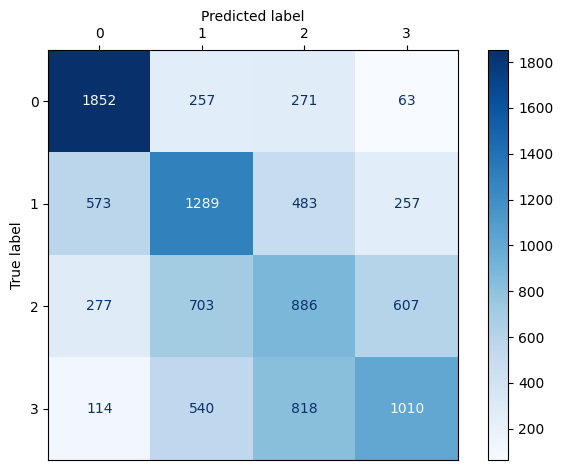
\includegraphics[width=0.5\linewidth]{images/trail_0002.png}
    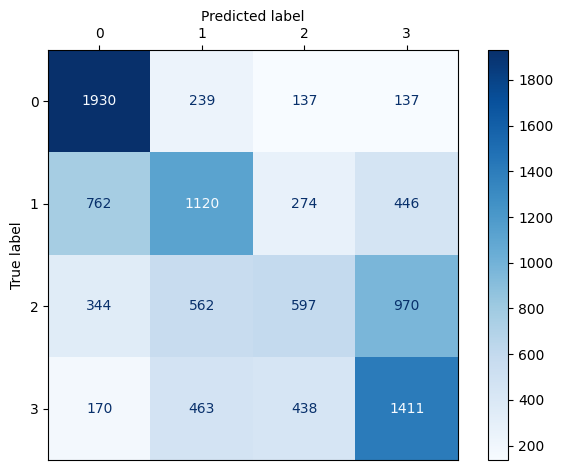
\includegraphics[width=0.5\linewidth]{images/trail_0005.png}
    \caption{Confusion matrix for Trail 0002 (top) and Trail 0005 (bottom)}
    \label{fig:confusion_matrix}
\end{figure}

\bibliographystyle{IEEEtran}
\bibliography{main}

\end{document}
